This section will contain a brief overview of the progress over the past 4 weeks. A summary of each researched subject is given. The full details are provided further in this report. Added sections are marked in \add{blue}. The text in black has been added with respect to the comments I received last time, but does contain major adjustments. The progress section concludes with the planning of the next weeks.


\section{Finished subjects}

\subsection{Input mapping}

The input mapping describes the transformation of physical inputs to model inputs. The physical set-up has two inputs which can pressurize each bellow individually. However, the dynamic model is based on forces and moments. Hence, we seek to find $p \mapsto F$. This mapping has been found by using the $\verb+Abaqus+$ finite element program. It has been shown that pressurizing both bellows equally, will result in the same deformation as attaching a force to the top of the actuator. Therefore a mapping between force and pressure can be found, by comparing the elongation.


\subsection{Stiffness determination}

The input mapping allows to determine the elongation stiffness $K_\epsilon$ and curvature stiffness $K_\kappa$. An inverse kinematic solver was made. This model is able to obtain elongation and curvature from the FEM simulations. The elongation and curvature were approximated using the constant curvature approach. The hyper-elastic stiffness model as formulated in \cite{Caasenbrood2020StiffnessModel} was used. This resulted in the following results,


\begin{figure}[H]
    \centering
\begin{minipage}{0.5\textwidth}
        \centering
        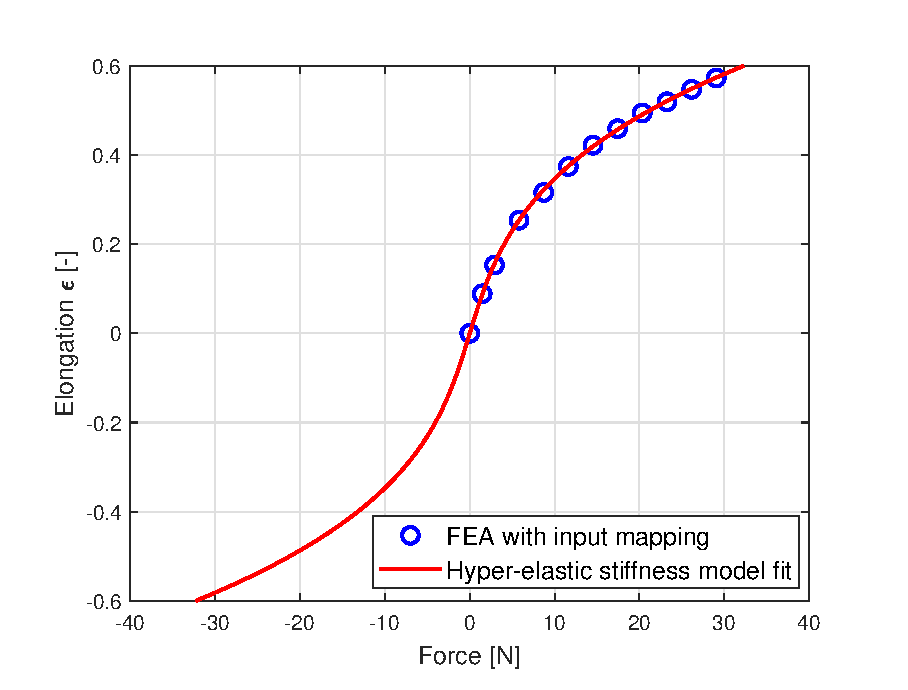
\includegraphics[width=\textwidth]{Figures/Chapter3/mappedforcevselongation.eps}
        \caption{Fitted stiffness model for elongation.}
    \end{minipage}\hfill
    \begin{minipage}{0.5\textwidth}
        \centering
        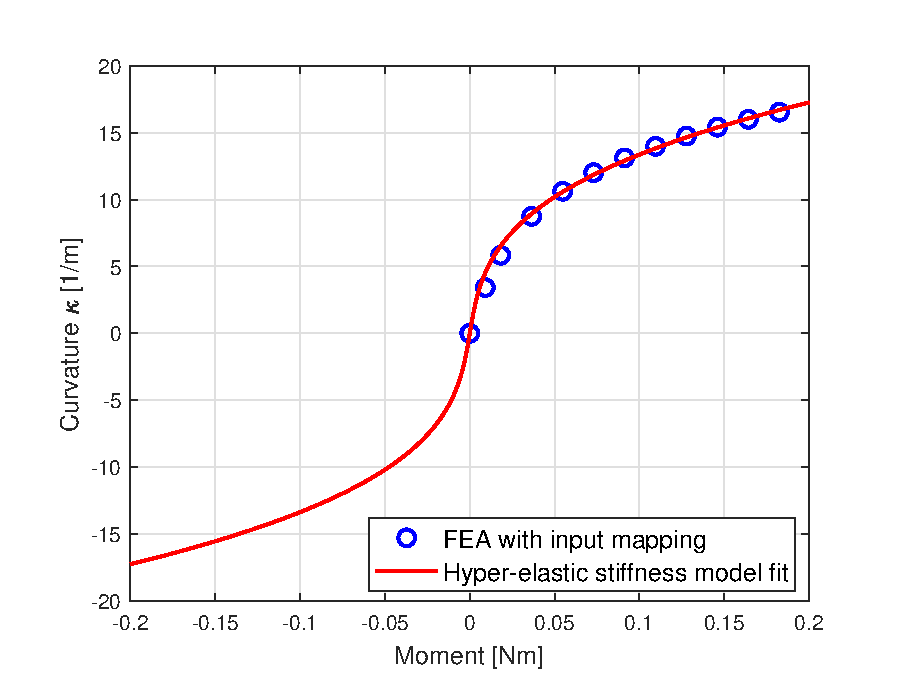
\includegraphics[width=\textwidth]{Figures/Chapter3/mappedmomentvscurvature.eps} 
        \caption{Fitted stiffness model for curvature.}
    \end{minipage}
\end{figure}


\section{Current research}

Now the non-linear stiffness has been obtained a start can be made with controller design. First a simplified non-linear model will be made in Matlab. This is done in Matlab since this is an environment I am more comfortable working with. After a controller has been found that is deemed good. I start implementation in C++.

The current research starts by implementing a forward dynamic model. First non-linear stiffness matrix $K$ is added. For now, mass matrix $M$ and damping matrix $D$ are constant, which gives,

\begin{equation}
    M = \begin{bmatrix} 0.0177 & 0 \\ 0 & 1.21e-5 \end{bmatrix}  ,  \hspace{20pt}  D = \begin{bmatrix} 0.1 & 0 \\ 0 & 0.02 \end{bmatrix} 
\end{equation}

where $M = \text{diag}(m, J_{xx})$ and $D = \text{diag}(d_\epsilon,d_\kappa)$. The mass matrix has been determined with $\verb+Abaqus+$. The damping matrix is arbitrary for now. With the previous found input mapping $H$, the system can be described by,

\begin{equation}
    M\Ddot{q} + C\dot{q} + K(q)q = Hp.
\end{equation}

Above can be rewritten to a system of first order differential equations using the state space formulation as,


\begin{equation}
     \begin{bmatrix} \dot{x_1} \\ \dot{x_2} \\\dot{x_3}  \\ \dot{x_4}  \end{bmatrix}   =      \begin{bmatrix} O_2 & I_2 \\ -M^{-1}K(q)  & -M^{-1}D \end{bmatrix}      \begin{bmatrix} x_1\\ x_2 \\x_3\\ x_4 \end{bmatrix}  +      \begin{bmatrix} O_2 \\ M^{-1}H   \end{bmatrix}       \begin{bmatrix} p_1\\ p_2   \end{bmatrix} 
\end{equation}

where $x = [\epsilon \hspace{4pt} \kappa \hspace{4pt} \dot{\epsilon} \hspace{4pt} \dot{\kappa}]^\top$.

Above has not been worked out further yet. Once this state-space is correctly implemented. An inverse dynamic analysis can be carried out, for which a model based controller can be designed. First a computed torque controller will be designed by using an inverted model. This might be extended with gravitational compensation.



\section{Planning for coming weeks}


\begin{itemize}
    \item Complete non linear state space model
    \item Include non-linear mass matrix
    \item Derive inverse dynamic model suitable for controller design
    \item Implement non-linear stiffness in C++ code
    \item When a controller has been made, implement it in C++
    \item First test, hopefully mid January
\end{itemize}